\documentclass[10pt,a4paper]{article}

\usepackage[utf8]{inputenc}
\usepackage[dutch]{babel}
\usepackage{amsmath}
\usepackage{amsfonts}
\usepackage{amssymb}
\usepackage{amsthm}
\usepackage{graphicx}
\usepackage{xcolor}
\usepackage{lipsum}
\usepackage{float}
\usepackage[framemethod=default]{mdframed}
\usepackage{todonotes}
\usepackage{xparse}
\usepackage{colortbl}
\usepackage{hyperref}
\usepackage{pgf}
\usepackage{tikz}
\usetikzlibrary{arrows,automata}

% Question command
\newtheorem{qtext}{Vraag}
\let\olddefinition\qtext
\renewcommand{\qtext}{\olddefinition\normalfont}

% Set text counters
\setcounter{qtext}{0}
\setcounter{section}{0}

\NewDocumentEnvironment{quest}{o}
 {\IfNoValueTF{#1}
   {\question\addcontentsline{toc}{subsection}{\protect\numberline{\thesubsection}Vraag}}
   {\question\addcontentsline{toc}{subsection}{\protect\numberline{\thesubsection}Vraag: #1}}%
   \ignorespaces}
 {\stepcounter{subsection}\endquestion}


% Define layout QuestionBox
\newmdenv[skipabove=7pt,
skipbelow=7pt,
rightline=false,
leftline=false,
topline=true,
bottomline=false,
linecolor=gray,
backgroundcolor=black!8,
innerleftmargin=5pt,
innerrightmargin=5pt,
innertopmargin=0pt,
leftmargin=0cm,
rightmargin=0cm,
linewidth=2pt,
innerbottommargin=5pt]{qbox}
\newenvironment{question}{\newpage\begin{qbox}\begin{qtext}}{\end{qtext}\end{qbox}}
\newtheorem{ttext}{Definitie}

% Theorem box
\newmdenv[skipabove=7pt,
skipbelow=7pt,
backgroundcolor=black!2,
linecolor=black,
rightline=false,
leftline=true,
topline=false,
bottomline=false,
innerleftmargin=5pt,
innerrightmargin=5pt,
innertopmargin=0pt,
leftmargin=0cm,
rightmargin=0cm,
linewidth=1pt,
innerbottommargin=5pt]{tbox}

\newenvironment{theorem}{\begin{tbox}\begin{ttext}}{\end{ttext}\end{tbox}}

\newenvironment{pushcenter}{\vspace{1mm}\begin{center}}{\vspace{1mm}\end{center}}

\setlength\parindent{0pt}

% Document info
\title{AUTOMATEN \\ \& \\ BEREKENBAARHEID}
\author{\emph{Jensen Bernard}}
\date{2016}

\begin{document}\sloppy

\pagenumbering{gobble}
\clearpage
\thispagestyle{empty}
\maketitle
\newpage

\begin{center}
	\emph{This page is intentionally left blank.}
\end{center}

% Preface
\newpage
\section*{Voorwoord}

Dit document bevat mogelijke examenvragen voor het vak \emph{Automaten en Berekenbaarheid}\footnote{Course G0P84a and G0P85a.}, gedoceerd aan de Katholieke Universiteit Leuven. In geen enkel geval wil dit document een vervanging zijn voor de cursus. De cursustekst, \emph{Automaten en berekenbaarheid}, geschreven door \emph{Bart Demoen}, is zeer goed en het is zeker aangeraden deze grondig door te nemen voor u begint aan de volgende vraagstukken.
Ik heb dit document opgesteld tijdens het studeren van het vak, om op deze manier een overzicht te hebben van mogelijke examenvragen die we kunnen verwachten in 2016. Vele vragen uit verschillende jaren komen zeer sterk overeen, daarom kan het zeker geen kwaad om deze extra aandacht te geven.
\\

Het is ook mogelijk dat er verwezen wordt naar delen uit de cursus. De meeste van deze verwijzingen zijn geschreven in December 2015. De meest recente versie was op dit moment de uitgave van 2013. Indien een nieuwere versie beschikbaar is, is het mogelijk dat de pagina's niet meer overeenstemmen. Aarzel niet om deze, zowel als mogelijke inhoudelijke fouten, aan te geven of aan te passen op Github.
\\

Ik heb vele studenten gehoord die vaak het nut niet inzien van dit vak, of dit totaal niet interessant vinden. Het is belangrijk eerst het voorwoord in de cursus eens te lezen, om een goed beeld te hebben van waar we nu eigenlijk mee bezig zijn. Indien u nog steeds van mening bent dat dit een enorm saai vak is, dan raad ik aan om ca. 2u te pauzeren om \emph{The Imitation Game}\footnote{Een film over Alan Turing, 2014.} te kijken. Kom daarna terug en alles zal veel interessanter lijken dan voordien.
\\

Thanks to \emph{Robin Haveneers} voor de hulp.
\\

\hfill \emph{Jensen Bernard}
\newpage
\tableofcontents
\newpage
\begin{center}
	\emph{This page is intentionally left blank.}
\end{center}

% CHAPTER 1: TALEN EN BEREKENBAARHEID
\newpage
\clearpage
\pagenumbering{arabic}

\section{Talen en Automaten}

\subsection{Inleiding}

	Dit hoofdstuk start met het kennismaken met talen en automaten. Het grootste deel van de leerstof uit dit hoofdstuk kan teruggevonden in de vragen, maar toch zijn er enkele puntjes die niet aan bod komen. Dit wil echter niet zeggen dat deze nooit zullen worden gevraagd op een examen. Ik raad aan de volgende secties achteraf eens te bekijken (sommige zijn misschien handig op voorhand):
	\begin{enumerate}
		\item Kennismaking - \emph{p4-p19}\footnote{Ook al komt dit niet expliciet aan bod, wanneer je de vragen beheerst, beheers je ook dit deel. Deze theorie komt overal terug. Je kan dit best lezen op voorhand.}
		\item Van reguliere expressie naar \emph{NFA} - \emph{p20}
		\item Doorsnede, complement en verschil van \emph{DFA's} - \emph{p15}
		\item Reguliere expressies en lexicale analyse - \emph{p47}
		\item Varianten van \emph{DFA's} - \emph{p49-p52}
		\item Equivalentie van \emph{CFG} en \emph{PDA} - \emph{p68}
		\item Algebra van contextvrije talen - \emph{p75}
	\end{enumerate}

\subsection{Equivalentie-relaties en -klassen}

	Aangezien velen problemen hadden met Myhill-Nerode relaties, is hier wat achtergrondinformatie om dit geheel beter te begrijpen. Stel dat we in het bezit zijn van vijf ballen. Hun volgorde is vast aangezien ze op een rij op tafel liggen. We kunnen dus spreken over $bal_i$ met $i \in \{1,2,3,4,5\}$. Deze duidt dan op de bal op de $i^{de}$ plaats.\\

	Laten we nu aannemen dat de oneven ballen rood zijn, de even ballen blauw. We kunnen op dit moment de ballen verdelen in groepen, namelijk de rode ($\{1,3,5\}$) en de blauwe ($\{2,4\}$). We gebruiken hier nu al (zonder het misschien te beseffen) equivalentie-relaties en -klassen!\\

	Laten we de equivalentierelatie $\sim_{kleur}$ defini\"eren, die nagaat of twee ballen dezelfde kleur hebben. Zo is bijvoorbeeld $bal_1 \sim_{kleur} bal_3$ waar, maar $bal_2 \sim_{kleur} bal_5$ niet!\\

	Een equivalentieklasse is dan eigenlijk de klasse (of verzameling) met alle elementen die voldoen aan een bepaalde equivalentierelatie waarvan \'e\'en element constant is. Zo kunnen we de volgende equivalentieklasses berekenen\footnote{Er bestaan er heel wat meer dan dit.}. We nemen even $i = bal_i$ voor een makkelijkere notatie.

	$$1_{\sim_{kleur}} = \{y|1 \sim_{kleur} y\} = \{1,3,5\}$$
	$$2_{\sim_{kleur}} = \{y|2 \sim_{kleur} y\} = \{2,4\}$$

	Houdt dit goed in het achterhoofd wanneer we gaan werken met Myhill-Nerode relaties aangezien deze verder bouwen op deze concepten. In deze cursus zijn $x$ en $y$ strings en worden deze als equivalent beschouwd op basis van (bv. een \emph{DFA}). Zo kunnen we de equivalentierelatie $\sim_{DFA}$ beschouwen die zegt dat

	$$x \sim_{DFA} y \iff \delta^*(q_s,x) = \delta^*(q_s,y)$$

	Een ander voorbeeld is $x \sim_L y$ indien $x \in L$ en $y \in L$.


\newpage

\begin{quest}[$A_{TM}$ is niet beslisbaar]
	Bewijs dat $A_{TM}$ niet beslisbaar is en steun daarbij niet op de stelling van \textit{Rice}. Zou het helpen als het toegelaten was op de stelling van \textit{Rice} te steunen? Is $A_{TM}$ herkenbaar? Co-herkenbaar?
\end{quest}

We hebben het hier over het acceptatieprobleem voor Turingmachines. We noemen de taal $A_{TM}$ met de volgende formele definitie. Informeel is elk element een tuple met het eerste element een ge\"encodeerde Turingmachine die de string $s$, het tweede element, accepteert.
\begin{center}
	$A_{TM} = \{ <M,s> |$ \textit{$M$ is een Turingmachine en} $ s \in L_M\}$
\end{center}

\subsubsection*{$A_{TM}$ is niet beslisbaar}
\begin{proof}
	Stel er bestaat een beslisser $B$ voor $A_{TM}$. De werking van $B$ kan op de volgende manier formeel gedefinieerd worden.

	\begin{pushcenter}
		$B(<M,s>)$ \textit{is accept als $M$ $s$ accepteert en anders reject}
	\end{pushcenter}

	$B$ weigert dus indien $M$ de input $s$ weigert of wanneer $M$ in een oneindige lus zit.
	We construeren nu een contradictie machine $C$ met de eigenschap om telkens het tegenovergestelde te accepteren (of te weigeren) van $B$. $C$ neemt daarbij enkel Machine $M$ als input en accept indien $M$ de string representatie van zichzelf accepteert. We kunnen dit op de volgende manier formeel schrijven.

	\begin{pushcenter}
		$\forall$ \textit{Turingmachine $M:$ $C(<M>) = \neg (B(<M,M>))$}
	\end{pushcenter}

	Daarbij is $\neg accept = reject$ en $\neg reject = accept$.  Neem nu voor $M$ hierboven $C$ zelf en vul deze in in $C$ en $B$ zelf. De volgende bewering komt tot stand.

	\begin{pushcenter}
		$C(<C>) = \neg (B(<C,C>))$
	\end{pushcenter}

	We zien dat $C$ zichzelf test. Indien $C$ zichzelf accepteert, dan is $\neg B(C,C) = C(C) = accept$. Aangezien $C$ $C$ accepteert, moet $B(C,C) = accept$ en dus $\neg B(C,C) = reject$. Contradictie.
	\\\\
	Conclusie: $C$ kan niet bestaan. Indien $B$ bestaat kan $C$ wel bestaan, dus $B$ bestaat ook niet. $A_{TM}$ is dus niet beslisbaar.
\end{proof}

\subsubsection*{De stelling van Rice}

\begin{theorem}[Stelling van Rice]
	Voor elke niet-triviale, taal-invariante eigenschap $P$ van Turingmachines geldt dat $Pos_P$ (en ook $Neg_P$) niet beslisbaar is.
\end{theorem}

Met deze stelling zouden we het hele bewijs kunnen inkorten. Door een niet-triviale, taal-invariante eigenschap $P$ te vinden van alle Turingmachines die $s$ herkennen, hebben we meteen aangetoond dat de taal in kwestie, $A_{TM}$ niet beslisbaar is.\footnote{Voor meer informatie over het bewijs, zie het laatste hoofdstuk.} Deze taal komt dan overeen met $Pos_P$. Een eigenschap van $<M,s>$ is bijvoorbeeld dat $M$ $s$ accepteert. $Pos_p = A_{TM}$ en dus is $A_{TM}$ niet beslisbaar.

\subsubsection*{$A_{TM}$ is herkenbaar}
\begin{proof}
	De herkenner $A$ voor $A_{TM}$ laat, met input $<M,s>$, $M$ lopen op $s$. Indien deze $M$ $s$ accepteert, dan accepteert $A$ zijn input. Indien deze de input $reject$, of gewoon niet stopt, dan zal $A$ deze ook niet accepteren. $A_{TM}$ is dus herkenbaar (ook hier zien we dat $A_{TM}$ niet beslisbaar is omdat deze kan blijven lopen).
\end{proof}

\subsubsection*{$A_{TM}$ is niet co-herkenbaar}
\begin{proof}
	$A_{TM}$ kan echter niet co-herkenbaar zijn. We bewijzen dit met contradictie. Indien $A_{TM}$ co-herkenbaar is, is deze dus herkenbaar en co-herkenbaar (zie vorig bewijs). Wanneer een taal deze beide eigenschappen bezit, is deze beslisbaar. Dit is een contradictie met het eerste bewijs.
\end{proof}

\begin{quest}[Recursie]
	Geef de conversieregels voor lambda-calculus, bespreek de stellingen van Church-Rosser en leg adh daarvan uit hoe je een recursieve functie in lambda-calculus kunt maken. Geef ook een voorbeeld dat we niet besproken hebben in de cursus.
\end{quest}

De regels en de stellingen van \emph{Church-Rosser} zijn in de vorige vraag al aan bod gekomen. We bekijken nu enkel recursieve functies in meer detail.\\

Om te kunnen werken met recursieve functies moeten we goed begrijpen wat vastepuntstheorie is. De uitleg uit het boek vind je op \emph{p154-p155}. Het is niet mogelijk deze in te korten aangezien deze uitleg al zeer compact is. Een ander voorbeeld dat we niet hebben besproken vind je hieronder terug. We gebruiken als voorbeeld $3^2$.

\begin{align*}
	\text{Pow} \enskip  3 \enskip 2 \enskip &= (Y\enskip H) \enskip 3 \enskip 2
	\\&= H \enskip (Y\enskip H) \enskip 3 \enskip 2
	\\&= (\lambda f. \enskip (\lambda xy. \enskip \text{IF} \enskip (= \enskip Y \enskip 0) \enskip 1 \enskip (* \enskip x \enskip (f \enskip x \enskip (- \enskip Y \enskip 1)))))(Y\enskip H) \enskip 3 \enskip 2
	\\&= (\lambda xy. \enskip \text{IF} \enskip (= \enskip Y \enskip 0) \enskip 1 \enskip (* \enskip x \enskip ((Y \enskip H) \enskip x \enskip (- \enskip Y \enskip 1)))) \enskip 3 \enskip 2
	\\&= * \enskip 3 \enskip ((Y \enskip H) \enskip 3 \enskip 1)
	\\&= * \enskip 3 \enskip (H \enskip (Y \enskip H) \enskip 3 \enskip 1)
	\\&= * \enskip 3 \enskip ((\lambda f. \enskip (\lambda xy. \enskip \text{IF} \enskip (= \enskip Y \enskip 0) \enskip 1 \enskip (* \enskip x \enskip (f \enskip x \enskip (- \enskip Y \enskip 1)))))(Y \enskip H) \enskip 3 \enskip 1)
	\\&= * \enskip 3 \enskip ((\lambda xy. \enskip \text{IF} \enskip (= \enskip Y \enskip 0) \enskip 1 \enskip (* \enskip x \enskip ((Y\enskip H)\enskip x\enskip (- \enskip Y \enskip 1)))) \enskip 3 \enskip 1)
	\\&= * \enskip 3 \enskip (* \enskip 3 \enskip ((Y \enskip H)\enskip 3 \enskip 0))
	\\&= * \enskip 3 \enskip (* \enskip 3 \enskip (H\enskip (Y \enskip H) \enskip 3 \enskip 0))
	\\&= * \enskip 3 \enskip (* \enskip 3 \enskip ((\lambda f \enskip (\lambda xy. \enskip \text{IF} \enskip (= \enskip Y \enskip 0)\enskip 1\enskip (* \enskip x\enskip (f \enskip x(-Y \enskip 1)))))(Y \enskip H)\enskip 3 \enskip 0))
	\\&= * \enskip 3 \enskip (* \enskip 3 \enskip ((\lambda xy. \enskip \text{IF} \enskip (=Y \enskip 0) \enskip 1(* \enskip x \enskip ((Y \enskip H)\enskip x\enskip (- \enskip Y \enskip 1))))\enskip 3 \enskip 0))
	\\&= * \enskip 3 \enskip (* \enskip 3 \enskip 1)
	\\&= * \enskip 3 \enskip 3
	\\&= 9
\end{align*}

\begin{quest}[Vraag 3]
Bewijs dat een eindige toestandsautomaat altijd een taal herkent die door een reguliere expressie wordt beschreven. Doe dat door een eindige toestandsautomaat te transformeren naar een gegeneraliseerde niet-deterministische eindige toestandsautomaat met slechts twee toestanden.\\
Kan voor een PDA ongeveer hetzelfde gedaan worden door een gegeneraliseerde PDA op te stellen?\\
\end{quest}

Voor we hier aan beginnen, defini\"eren we de \emph{GNFA} als volgt:
\begin{theorem}[GNFA]
Een GNFA (gegeneraliseerde niet-deterministische eindige automaat) is een eindige toestandsmachine met de volgende wijzigingen en beperkingen:
\begin{enumerate}
\item Er is slechts 1 eindtoestand $\neq$ starttoestand
\item Er is juist 1 boog van de starttoestand naar elke andere toestand en er komen geen pijlen aan (buiten de startpijl)
\item Er is juist 1 boog van elke toestand naar de eindtoestand, maar er vertrekken geen pijlen vanuit de eindtoestand
\item Tussen elke andere 2 toestanden is er juist 1 boog in beide richtingen
\item Er is juist 1 boog van elke andere toestand naar zichzelf
\item De bogen hebben als label een reguliere expressie
\end{enumerate}
\end{theorem}
In wat volgt bewijzen we dat een eindige toestandsautomaat altijd een taal herkent die door een reguliere expressie wordt beschreven. We volgen volgend stappenplan:
$$ \text{NFA} \rightarrow \text{GNFA} \rightarrow \text{GNFA met 2 toestanden} \rightarrow \text{reguliere expressie} $$
In de opgave spreken ze van een ``eindige toestandsautomaat'', we gaan er hier echter vanuit dat we starten vanaf een NFA. Dit mag vermits elke DFA omgezet kan worden naar een NFA.

\begin{proof}
\subsubsection*{(a) NFA $\rightarrow$ GNFA}
We kunnen onze NFA omzetten naar een GNFA als volgt:
\begin{enumerate}
\item Maak een nieuwe starttoestand en een nieuwe (unieke) eindtoestand
\item Teken $\epsilon$-bogen van de nieuwe begintoestand naar de oude begintoestand en van elke oude eindtoestand naar de nieuwe eindtoestand.
\item Teken ontbrekende bogen met een $\phi$.
\item Als er tussen twee toestanden twee of meer parallele gerichte bogen zijn, neem die dan samen met als label de unie van de labels van de parallelle bogen.
\end{enumerate}
Deze omzetting van NFA naar GNFA verandert de taal niet. We doen namelijk enkel correct manipulaties van de NFA.\\
Nu we een GNFA geconstrueerd hebben moeten we deze reduceren naar een GNFA met 2 toestanden.

\subsubsection*{(b) Reduceren van de GNFA}
Dit doen we door herhaaldelijk een willekeurige toestand X verschillend van de start- of eindtoestand te kiezen en deze knoop de verwijderen als volgt:
\begin{enumerate}
\item Kies toestanden A en B zodat er bogen zijn van: 
\begin{itemize}
\item A naar B met label $E_4$
\item A naar X met label $E_1$
\item X naar zichzelf met label $E_2$
\item X naar B met label $E_3$
\end{itemize}
\item Vervang het label op de boog van A naar B door $E_4 | E_1 E_2^* E_3$.
\item Doe dit voor alle koppels A en B
\item Verwijder de knoop X met alle bogen die erin toekomen of vertrekken.
\end{enumerate}
Indien er geen toestanden meer zijn, ga naar stap (c).

\subsubsection*{(c) Bepaal RE}
De GNFA heeft nu exact 2 toestanden (een start- en eindtoestand) met daartussen 1 boog. Deze boog heeft nu een reguliere expressie als label. Dit is de reguliere expressie die dezelfde taal bepaald als de oorspronkelijke NFA.
\end{proof}

\subsubsection*{(d) Extra}
In wat volgt bewijzen we nog dat de reductie met 1 toestand de verzameling aanvaarde strings niet verandert. Hiervoor moeten we aantonen dat indien s aanvaard werd voor de reductie, deze ook na de reductie aanvaard wordt (1) en indien s niet aanvaard werd voor de reductie, deze na de reductie ook niet aanvaard wordt (2).\\
\subsubsection*{(1)}
\begin{proof}
Als s aanvaard werd door een pad zonder X, wordt s nog steeds aanvaard: paden zonder X blijven namelijk bestaan. Als het pad X bevat zijn er toestanden A en B zodat $AX^n B$ een opeenvolging van toestanden is. De reguliere expressie op bogen AX,XX en XB zijn $E_1$, $E_2$ en $E_3$ en bijgevolg kost van A naar B gaan langs X een stuk string van de vorm $E_1  (E_2)^* E_3$. Deze reguliere expressie staat ook in de boog AB van de nieuwe GNFA.
\end{proof}
\subsubsection*{(2)}
\begin{proof}
Als s aanvaard wordt door de gereduceerde GNFA dan bevat het acceptatiepad uiteraard alleen toestanden verschillend van X. Op een boog AB staat de reguliere expressie $E_4 | E_1 (E_2)^* E_3$. Die gebruiken betekent  een stukje string uitgeven dat voldoet aan $E_4$ of aan $E_1 (E_2)^* E_3$. Dus in de originele GNFA komt dit overeen met ofwel de boog AB volgen ofwel AX,XX (een aantal keer) en XB.\\
Dus als de string aanvaard wordt door de gereduceerde GNFA wordt hij ook aanvaard door de originele GNFA.
\end{proof}

\subsubsection*{(e) Kan dit ook met een PDA?}
Dit is mogelijk aangezien we bij gewone FSM's labels samen nemen in een reguliere expressie. Een PDA kan dit ook doen, aangezien we meerdere karakters in \'e\'en enkele keer op de stapel kunnen schrijven (of verwijderen).

\begin{question}
Geef een precieze formulering van het pompend lemma voor reguliere talen en een bewijs ervan. Geef voorbeelden waarbij je laat zien hoe je dat lemma gebruikt om te bewijzen dat een gegeven taal regulier is en om te bewijzen dat een gegeven taal niet regulier is.
\end{question}

We beginnen met dit alles intu\"itief te bekijken:\\
Stel je hebt een reguliere taal met oneindig veel strings. Er bestaat een DFA voor L met $N = \#Q$ toestanden. Neem nu een string in L die langer is dan N en begin de tocht van starttoestand naar eindtoestand. Vermits er maar N toestanden zijn en je string meer dan N lang is en je bij elke overgang juist 1 symbool achterlaat, moet je op je weg naar de eindtoestand minstens 1 toestand S 2 of meer keer tegenkomen. Je hebt dus ergens een kring gemaakt. In deze string werd een substring van de oorspronkelijke string gebruikt.\\
We defini\"eren nu het pompend lemma voor reguliere talen.

\begin{theorem}[Pompend lemma voor reguliere talen]
Voor een reguliere taal L bestaat een pomplengte $d$, zodanig dat als $s \in L$ en $|s| \geq d$, dan bestaat er een verdeling van $s$ in stukken x,y en z zodanig dat s = xyz en:
\begin{enumerate}
\item $\forall i \geq 0 : xy^iz \in L$
\item $|y| > 0$
\item $|xy| \leq d$
\end{enumerate}
\end{theorem}

In wat volgt bewijzen we deze stelling:

\begin{proof}
Neem een DFA die L bepaalt. Neem d = $\#Q+1$.\\
Neem een willekeurige string $s = a_1a_2 \hdots a_n$ met $n \geq d$. \\
Beschouw de accepterende sequentie van toestanden ($q_s = q_1,q_2,\hdots,q_f)$ voor $s$; die heeft lengte strikt groter dan $d$, dus zijn er bij de eerste $d$ zeker twee toestanden gelijk (omdat er maar $d-1$ toestanden zijn).\\
Stel dat $q_i$ en $q_j$ gelijk zijn met $i<j \leq d$ dan nemen we $x=a_1a_2\hdots a_i$ en $y=a_{i+1} \hdots a_j$ en $z$ de rest van de string. Alles volgt nu direct.
\end{proof}

Met het pompend lemma kan je \emph{niet} bewijzen dat een taal regulier is. De stelling zegt immers niet dat als het pompend lemma geldt de taal sowieso regulier is. Er kunnen nog andere condities van een reguliere taal niet voldaan zijn.
Je kan echter wel aantonen dat een taal niet-regulier is door een contradictie te bewijzen met de stelling hierboven.\\
Een soortgelijk bewijs heeft steeds de volgende structuur:
\begin{itemize}
\item Kies een willekeurig getal als pomplengte d
\item bestaat er een string langer dan d
\item waarvoor \textbf{elke} opdeling pompen verhinderd
\end{itemize}

Algemeen voorbeeld:
\begin{proof}
Stel dat er voor $L= \{a^nb^n | n \in \mathbb{N}\}$ een pomplengte $d$ bestaat. Beschouw dan de string $s=a^db^d$. Neem een willekeurige opdeling can $s=xyz$ met $|y| > 0$ dan zijn er 3 mogelijkheden:
\begin{enumerate}
\item y bevat alleen a's: dan bevat xyyz meer a's dan b's en zit deze string dus niet in $L$
\item y is van de vorm $a^ib^j$ met $i \neq 0, j \neq 0$: dan bevat xyyz niet alle a's voor de b's, en zit de string dus niet in L
\item y bevat alleen b's: dan bevat xz meer a's dan b's en zit de string dus niet in L
L kan dus niet regulier zijn.
\end{enumerate}
\end{proof}


\begin{quest}[Myhill-Neroderelaties (a)]
  Geef de definitie van een Myhil-Nerode relatie over een taal \emph{L}, of zoals we noteren een \emph{MN(L)}-relatie. \\
  Bewijs vervolgens dat een \emph{MN(L)}-relatie bestaat als en slechts als \emph{L} regulier is. Bestaat er voor een taal \emph{L} soms meer dan één \emph{MN(L)}-relatie? Hoe zit het met \emph{MN(L)}-relaties bij \emph{PDA’s}?
\end{quest}

\subsubsection*{Definitie}

\begin{theorem}[Myhill-Nerode Relatie]
  Wanneer een equivalentierelatie $\sim_{DFA}$ voldoet aan de volgende voorwaarden:
  \begin{enumerate}
    \item $\forall x, y \in \Sigma^*, a \in \Sigma : x \sim_{DFA} y \rightarrow xa \sim_{DFA} ya$ (m.a.w. rechts congruent)
    \item $\sim_{DFA}$ verfijnt $\sim_L$ (m.a.w. $x \sim_{DFA} y \rightarrow x \sim_L y$)
    \item $\sim_{DFA}$ heeft een eindige index (m.a.w. het aantal equivalentieklassen van $\sim_{DFA}$ is eindig)
  \end{enumerate}
  Dan spreken we van een Myhill-Nerode relatie voor $L$ (oftewel $MN(L)$) indien de \emph{DFA} de taal \emph{L} bepaalt.
\end{theorem}

Dit heeft zin aangezien de drie eigenschappen verwijzen naar \emph{L}. Hierdoor kunnen we, vertrekkend van een \emph{DFA} die \emph{L} accepteert, een $MN(L)$ relatie construeren op $\Sigma^*$.

\subsubsection*{L is regulier}

We kunnen ook het omgekeerde doen en dus, vertrekkende uit $MN(L)$ een \emph{DFA} construeren zodat $L_{DFA} = L$.

\begin{theorem}
  Gegeven een taal \emph{L} over $\Sigma$ en een $MN(L)$-relatie $\sim$ op $\Sigma^*$, dan definieert $(Q,\Sigma,\delta,q_s,F)$ een \emph{DFA} die \emph{L} bepaalt, waarbij
  \begin{enumerate}
    \item $Q = \{x_{\sim}|x \in \Sigma^*\}$\footnote{Hier is dus $x_{\sim}$ de toestand waar alle strings $x$ (of equivalent aan $x$) in terecht komen.}
    \item $q_s = \epsilon_{\sim}$
    \item $F = \{x_{\sim}|x \in L\}$
    \item $\delta(x_{\sim},a) = (xa)_{\sim}$\footnote{We hebben $x_{\sim}$ in punt 1 gedefinieerd als $\delta^*(q_s,x)$ dus deze is gelijk aan $\delta^*(q_s,xa) = (xa)_{\sim}$.}
  \end{enumerate}
\end{theorem}

\begin{proof}
  Dat $\delta$ goed gedefinieerd is, kan je bewijzen door gebruik te maken van de rechtse congruentie van $\sim$. Verder zijn alle andere ingredi\"enten van de \emph{DFA} duidelijk, in het bijzonder ook dat $Q$ (en $F$) slechts een eindig aantal toestanden bevat. We moeten enkel nog bewijzen dat $L_{DFA} = L$. Stel dat $x$ geaccepteerd wordt door de \emph{DFA}.
  $$x \in L_{DFA} \iff \delta(q_s, x) \in F$$
  Uit de definitie van de \emph{DFA} kunnen we zeggen dat $q_s = \epsilon_{\sim}$. Dus $\delta(\epsilon_{\sim},x) \in F$. De toestand waarin string $x$ komt kunnen we schrijven als $x_{\sim}$ (zie punt 1). We kunnen dus het volgende besluiten.
  $$\delta(\epsilon_{\sim},x) \in F \iff x_{\sim} \in F$$
  Aangezien dit laatste geldt, kunnen we zeggen dat $x \in L$. Er bestaat dus een \emph{DFA} voor \emph{L}, dus \emph{L} is regulier.
\end{proof}

\subsubsection*{Meerdere MN(L) relaties}

Dit is zeker mogelijk aangezien er ook oneindig veel (niet-isomorfe) \emph{DFA's} bestaan die taal \emph{L} aanvaarden.

\subsubsection*{Hoe zit het met een PDA?}

Het principe blijft volledig hetzelfde. Echter was het bij een \emph{DFA} genoeg om enkel ervoor te zorgen dat de toestand hetzelfde was voor twee strings $x$ en $y$ om deze als equivalent te beschouwen. Indien we specifiek naar een \emph{PDA} kijken, dan moeten we een toestand niet individueel bekijken, maar in combinatie met de stack. Twee strings $x$ en $y$ zijn dan equivalent indien zowel de toestand waarin ze eindigen, als de stack, gelijk zijn.\\

Het probleem is echter dat de stack oneindig veel mogelijkheden heeft en dus heeft de equivalentierelatie geen eindige index. Het is dus geen Myhill-Neroderelatie, wel een equivalentierelatie.

\begin{quest}[Myhill-Neroderelaties (b)]
  Reconstrueer de details van het verhaal van Myhill-Nerode. Leg uit alle stellingen uit: \emph{DFA} bepaalt een Myhill-Neroderelatie. Elke Myhill-Neroderelatie bepaalt een \emph{DFA}; twee isomorfe \emph{DFA's} bepalen dezelfde Myhill-Nerode-relatie. Het supremum van twee Myhill-Neroderelaties is een Myhill-Neroderelatie. Argumenteer ook het verband tussen de minimale \emph{DFA} voor een reguliere taal \emph{L} en de grofste \emph{MN(L)}-relatie.
  Kan je ook een Myhill-Neroderelatie construeren voor een \emph{NFA}? Wat krijg je dan met minimalisatie?
\end{quest}

Deze vraag is zeer groot. De eerste twee puntjes \emph{Elke DFA bepaalt een Myhill-Neroderelatie} en \emph{Elke Myhill-Neroderelatie bepaalt een DFA} kun je uitleggen met het antwoord op de vorige vraag.

\subsubsection*{Twee isomorfe DFA's}

\begin{proof}
  Stel dat we twee isomorfe \emph{DFA's} hebben die de taal \emph{L} bepalen ($DFA_1$ en $DFA_2$). Dit wil zeggen dan er een \'e\'en op \'e\'en relatie is tussen hun toestanden (volgt uit de definitie van isomorfisme). Stel dat $x$ in $DFA_1$ eindigt in $q_{1,x}$ met $q_{1,x} = \delta_1(q_{1,s},x) = q_1‡$ indien $q_{1,s}$ de starttoestand is van $DFA_1$. Uit de definitie van isomorfisme volgt dat $\delta_2(q_{2,s},x) = q_{2,x} = q_2$ met $q_{2,s}$ de starttoestand van $DFA_2$ en dat $q_2$ equivalent is met $q_1$. Beide relaties zijn dus equivalent.
\end{proof}

\subsubsection*{Supremum van twee MN(L) relaties}

Gegeven een reguliere taal \emph{L} en twee $MN(L)$-relaties $\sim_1$ en $\sim_2$. We kunnen van die twee relaties het supremum beschouwen in de tralie van equivalentierelaties of partities. Het supremum $\sim_{sup}$ is de fijnste relatie die groffer is dan beide relaties en die dus bevat, namelijk:

\begin{theorem}
  $x \sim_{sup} y$ is de transitieve sluiting van $(x \sim_1 y)$ of $(x \sim_2 y)$.
\end{theorem}

\begin{theorem}
  Het supremum van twee $MN(L)$-relaties is ook een $MN(L)$-relatie: als $\sim_1$ en $\sim_2$ $MN(L)$-relaties zijn, dan is het supremum $\sim_{sup}$ van $\sim_1$ en $\sim_2$ ook een $MN(L)$-relatie.
\end{theorem}

\begin{proof}
  Zie boek \emph{p40} voor de formele notaties. Het komt er op neer om het supremum voluit te schrijven en dan de drie hoofdeigenschappen van een Myhill-Neroderelatie aan te tonen (door te termen terug op te splitsen en samen te nemen).
\end{proof}

\subsubsection*{Minimale DFA}

Minimale \emph{DFA} wijst op het minimaal aantal toestanden. Aangezien $x \sim y$ indien ze in beide toestand eindigen, zijn er minder equivalentierelaties. Aangezien het universum verdeeld wordt in equivalentieklassen (\'e\'en klasse per equivalentierelatie) zullen de klassen dus ook zo groot mogelijk zijn. Dit is de definitie van \emph{grofste}.

\subsubsection*{MN(L) voor een NFA}

Aangezien we een \emph{DFA} kunnen opstellen van een \emph{NFA} kunnen we ook een $MN(L)$-relatie opstellen. Dit zijn er echter heel wat, aangezien we verschillende \emph{DFA's} kunnen opstellen die equivalent zijn aan de gegeven \emph{NFA}.

\begin{quest}[Vraag 7]
  Geef alle stappen (stellingen \& bewijzen) om aan te tonen dat alle minimale DFA's die dezelfde taal bepalen isomorf zijn.
\end{quest}

De twee voorgaande vragen zijn belangrijk voor deze vraag. Dit antwoord baseert zich op voorgaande theori\"en. Ik zou ze niet allemaal geven, maar als hij doorvraagt moet je ze wel kennen.

\begin{proof}

  Neem twee minimale DFA's voor eent taal L. We zullen bewijzen dat ze isomorf zijn. Beiden hebben hetzelfde aantal toestanden $N$ - anders was \'e\'en van de twee niet minimaal. Neem nu het supremum van die twee DFA's: je krijgt een DFA met opnieuw $N$ toestanden, want meer kan niet, maar ook minder niet.

  In termen van de $MN(L)$-relaties door de drie betrokken DFA's ge\"induceerd betekent dat dat die drie relaties identiek zijn. In termen van de drie DFA's betekent het dat ze alle drie isomorf zijn.

  Pas nu weten we zeker dat de minimisatieprocedure eindigt met een uniek resultaat (op isomorfisme na).
\end{proof}

De karakterisatie van de $MN(L)$-relatie die hoort bij de minimale DFA is redelijk eenvoudig:
$$x \sim_{min} y \iff \forall s \in \Sigma^*(xs \in L \iff ys \in L)$$
In essentie zegt dit: als twee toestanden f-gelijk zijn, dan zijn ze identiek.

\begin{quest}[Vraag 8]
Geef een precieze formulering van het pompend lemma voor context-vrije talen en een bewijs ervan. Geef voorbeelden waarbij je laat zien hoe je dat lemma gebruikt om te bewijzen dat een gegeven taal context-vrij is en om te bewijzen dat een gegeven taal niet context-vrij is.
\end{quest}

Het pompend lemma voor contextvrije talen gaat als volgt:
\begin{theorem}[Pompend lemma voor contextvrije talen]
Voor een contextvrije taal \emph{L} bestaat een getal $P$ (de pomplengte) zodanig dat elke string $s$ van \emph{L} met lengte minstens $p$ kan opgedeeld worden in vijf stukken $u$,$v$,$x$,$y$ en $z$ uit $\Sigma^*$ zodanig dat $s = uvxyz$ en
\begin{enumerate}
\item $\forall i \geq 0 : uv^ixy^iz \in L$
\item $|vy| > 0$
\item $|vxy| \leq p$
\end{enumerate}
\end{theorem}

Dit is te bewijzen als volgt:
\begin{proof}
Eerst en vooral gaan we onze \emph{CFG} in Chomsky normaalvorm zetten. Dit is een meer restrictieve vorm:
\begin{theorem}[Chomsky Normaal Vorm]
Een \emph{CFG} heeft de Chomsky Normaal Vorm als elke regel \'e\'en van de volgende vormen heeft:
\begin{enumerate}
\item $A \rightarrow BC$
\item $A \rightarrow \alpha$
\item $S \rightarrow \epsilon$
\end{enumerate}
Hierin is $\alpha$ een eindsymbool, $A$ een niet-eindsymbool en $B,C$ niet-eindsymbolen verschillend van het startsymbool.
\end{theorem}
Nu dat de \emph{CFG} is omgezet heeft elke regel ofwel twee ofwel geen niet-terminalen aan de rechterkant. Stel nu $n$ gelijk aan het aantal niet-eindsymbolen in de CFG.\\[0.5cm]

Voor een bepaalde string $s$ uit \emph{L} bestaat er steeds een parse tree. Als je uit deze parse tree de onderste takken wegsnoeit hou je een volledige binaire boom over want de \emph{CFG} staat in Chomsky Normaal Vorm. De hoogte van de boom is minstens gelijk aan $log_2(|s|)$. Het langste enkelvoudige pad van de wortel bevat dus minstens $log_2(|s|)+1$ knopen en als we $s$ lang genoeg kiezen, dan is $log_2(|s|)+1$ groter dan $n$ en bijgevolg moet er op dat langste pad minstens \'e\'en niet-eindsymbool (neem $X$) herhaald worden.\\[0.5cm]

Neem de laagste $X$ ($X_2$) en zijn dichtste herhaling ($X_1$) op dat pad. $X$ is zeker verschillen van het startsymbool. We kunnen nu een afleiding construeren van de vorm:
$$ S \Rightarrow^* u X_2 z \Rightarrow^* u v X_1 y z \Rightarrow^* uvxyz  $$
In deze afleiding zijn $u,v,x,y,z$ strings uit $\Sigma^*$ en bovendien zijn $v$ en $y$ niet tegelijkertijd leeg, want dan zou men uit $X$ zichzelf kunnen afleiden en dat kan niet wegens de vorm van de grammatica. \\[0.5cm]

Vermits bovenstaande afleiding geldig is, zijn
$$ S \Rightarrow^* u X_2 z \Rightarrow^* u x z  $$
en
$$ S \Rightarrow^* u X z \Rightarrow^* u v X y z \Rightarrow^* u v v x y y z  $$
dat ook. \\[0.5cm]

We hebben nu de eerste twee puntjes van de de stelling al bewezen indien er strings gekozen worden die langer zijn dan $2^{(n-1)}$. Dit is onze pomplengte $p$. $vxy$ wordt afgeleid vanuit $X$ met een parse tree die kleiner is dan $n$. De parse tree heeft dus hoogstens $2^{n-1}$ bladeren en die corresponderen juist met $vxy$. Hiermee is het derde puntje ook bewezen.

\end{proof}

\begin{quest}[Vraag 9]
Geef het algoritme om een CFG naar zijn PDA om te zetten en bewijs de correctheid hiervan.
Volgens een constructie in de cursus worden meerdere elementen per keer gepushed, waarom mag dit?
\end{quest}

\subsubsection*{Algoritme}

We stellen de PDA op door middel van 3 toestanden. De starttoestand $q_s$, de eindtoestand $q_f$ en een hulptoestand $x$. We trekken slechts \'e\'en boog van $q_s$ naar $x$: die kijkt niet naar de string of stapel, en een marker $\$$ op de stapel, samen met het beginsymbool (meestal $E$). Er is ook slechts \'e\'en boog van $x$ naar $q_f$: die consumeert niks van de string en haalt de marker $\$$ van de stapel. De andere bogen gaan van $x$ naar $x$, de labels corresponderen met:
\begin{enumerate}
	\item de symbolen uit het invoeralfabet: voor elke $\alpha \in \Sigma$, is er een boog met label $\alpha, \alpha \rightarrow \epsilon$; die bogen beteken dus: als de top van de stapel gelijk is aan het eerste symbool van de string, consumeer dan beide.
	\item de regels van de grammatica: voor elke regel $X \rightarrow \gamma$ is er een label $\epsilon,X \rightarrow \gamma$; die bogen betekenen dus: als de top van de stapel een niet-eindsymbool $X$ is, vervan het door de rechterkant $\gamma$ van een regel in de grammatica waarvan $X$ de linkerkant is; $\gamma$ is een rij eind- en niet-eindsymbolen.
\end{enumerate}

\subsubsection*{Correctheid}

Het algoritme is steeds correct, aangezien het hetzelfde werkt dan we intuitief zouden doen. Het vult steeds een nieuwe expressie in en verwijderd eventuele atomen.\footnote{Ik heb geen flauw idee, send me the answer.}

\subsubsection*{Meerdere elementen pushen}

Het is mogelijk om meerdere elementen in \'e\'en stap pushen, aangezien dit overeenkomt met meerdere $\epsilon, \epsilon \rightarrow \alpha$ stappen.
\begin{question}
Vertel alles wat je weet i.v.m. de Chomsky-hierarchie binnen de 5 minuten. \\
Zijn de talen van een TM beslisbaar en wat is de tijdscomplexiteit doorheen de Chomsky-hierarchie.
\end{question}
\todo{TODO}

\newpage


\section{Talen en Berekenbaarheid}

\subsection{Inleiding}

\vspace{3mm}
In dit hoofdstuk, Talen en Berekenbaarheid\footnote{Dit is hoofdstuk 3 in de cursus (versie 2013).}, zal er dieper worden ingegaan op Turingmachines en de werking ervan. Na het instuderen van dit hoofdstuk is het best om onderstaande vragen op te lossen. Het zijn niet zo veel vragen, maar ze bevatten steeds een redelijk groot deel van de leerstof (vaak ook verschillende stukken gecombineerd). De vragen die volgen zijn alle vragen die al eens gesteld zijn. Deze komen echter elk jaar terug. Concreet wil dit zeggen dat als al deze vragen gekend zijn een goed resultaat verwacht kan worden.\\

Dit wil echter niet zeggen dat het onmogelijk is om een andere vraag te krijgen. In de volgende sectie staat een kleine opsomming van delen uit het hoofdstuk die (tot nu toe) niet aan bod gekomen zijn tijdens de examens\footnote{Het gaat hier enkel over het mondeling examen, niet over testen.}. Er bestaat echter een kleine kans dat hij zijn vragen veranderd, wat wil zeggen dat ook deze delen gekend moeten zijn. In het algemeen zijn de vragen uit dit document echter goed genoeg.\\

In een andere repo kan je ook een implementatie van een Turingmachine terugvinden (geschreven in Haskell). De link vind je in de readme van deze repo. Dit kan een dieper inzicht geven op hoe zo een machine werkt.

\subsection{Extra lectuur}

De volgende secties dit hoofdstuk zijn tot nu toe nog nooit aan bod gekomen op het examen, maar moeten wel gekend zijn. De pagina's komen overeen met de publicatie van 19 november 2013\footnote{De meeste recente versie in 2016.}.

\begin{enumerate}
	\item Basiswerking van een Turingmachine - \emph{p82-p86}
	\item Er bestaat een niet herkenbare taal - \emph{p87}
	\item Universele Turingmachines - \emph{p95}
	\item Verband met reguliere talen - \emph{p100}
	\item $Regular_{TM}$ en $EQ_{TM}$ - \emph{p105}
	\item Aftelbaar - \emph{p110}
	\item The Post Correspondence Problem - \emph{p113-p116}
	\item Recursieve functies - \emph{p122-p125}
	\item De bezige bever - \emph{p126-p127}
\end{enumerate}

\begin{quest}[$A_{TM}$ is niet beslisbaar]
	Bewijs dat $A_{TM}$ niet beslisbaar is en steun daarbij niet op de stelling van \textit{Rice}. Zou het helpen als het toegelaten was op de stelling van \textit{Rice} te steunen? Is $A_{TM}$ herkenbaar? Co-herkenbaar?
\end{quest}

We hebben het hier over het acceptatieprobleem voor Turingmachines. We noemen de taal $A_{TM}$ met de volgende formele definitie. Informeel is elk element een tuple met het eerste element een ge\"encodeerde Turingmachine die de string $s$, het tweede element, accepteert.
\begin{center}
	$A_{TM} = \{ <M,s> |$ \textit{$M$ is een Turingmachine en} $ s \in L_M\}$
\end{center}

\subsubsection*{$A_{TM}$ is niet beslisbaar}
\begin{proof}
	Stel er bestaat een beslisser $B$ voor $A_{TM}$. De werking van $B$ kan op de volgende manier formeel gedefinieerd worden.

	\begin{pushcenter}
		$B(<M,s>)$ \textit{is accept als $M$ $s$ accepteert en anders reject}
	\end{pushcenter}

	$B$ weigert dus indien $M$ de input $s$ weigert of wanneer $M$ in een oneindige lus zit.
	We construeren nu een contradictie machine $C$ met de eigenschap om telkens het tegenovergestelde te accepteren (of te weigeren) van $B$. $C$ neemt daarbij enkel Machine $M$ als input en accept indien $M$ de string representatie van zichzelf accepteert. We kunnen dit op de volgende manier formeel schrijven.

	\begin{pushcenter}
		$\forall$ \textit{Turingmachine $M:$ $C(<M>) = \neg (B(<M,M>))$}
	\end{pushcenter}

	Daarbij is $\neg accept = reject$ en $\neg reject = accept$.  Neem nu voor $M$ hierboven $C$ zelf en vul deze in in $C$ en $B$ zelf. De volgende bewering komt tot stand.

	\begin{pushcenter}
		$C(<C>) = \neg (B(<C,C>))$
	\end{pushcenter}

	We zien dat $C$ zichzelf test. Indien $C$ zichzelf accepteert, dan is $\neg B(C,C) = C(C) = accept$. Aangezien $C$ $C$ accepteert, moet $B(C,C) = accept$ en dus $\neg B(C,C) = reject$. Contradictie.
	\\\\
	Conclusie: $C$ kan niet bestaan. Indien $B$ bestaat kan $C$ wel bestaan, dus $B$ bestaat ook niet. $A_{TM}$ is dus niet beslisbaar.
\end{proof}

\subsubsection*{De stelling van Rice}

\begin{theorem}[Stelling van Rice]
	Voor elke niet-triviale, taal-invariante eigenschap $P$ van Turingmachines geldt dat $Pos_P$ (en ook $Neg_P$) niet beslisbaar is.
\end{theorem}

Met deze stelling zouden we het hele bewijs kunnen inkorten. Door een niet-triviale, taal-invariante eigenschap $P$ te vinden van alle Turingmachines die $s$ herkennen, hebben we meteen aangetoond dat de taal in kwestie, $A_{TM}$ niet beslisbaar is.\footnote{Voor meer informatie over het bewijs, zie het laatste hoofdstuk.} Deze taal komt dan overeen met $Pos_P$. Een eigenschap van $<M,s>$ is bijvoorbeeld dat $M$ $s$ accepteert. $Pos_p = A_{TM}$ en dus is $A_{TM}$ niet beslisbaar.

\subsubsection*{$A_{TM}$ is herkenbaar}
\begin{proof}
	De herkenner $A$ voor $A_{TM}$ laat, met input $<M,s>$, $M$ lopen op $s$. Indien deze $M$ $s$ accepteert, dan accepteert $A$ zijn input. Indien deze de input $reject$, of gewoon niet stopt, dan zal $A$ deze ook niet accepteren. $A_{TM}$ is dus herkenbaar (ook hier zien we dat $A_{TM}$ niet beslisbaar is omdat deze kan blijven lopen).
\end{proof}

\subsubsection*{$A_{TM}$ is niet co-herkenbaar}
\begin{proof}
	$A_{TM}$ kan echter niet co-herkenbaar zijn. We bewijzen dit met contradictie. Indien $A_{TM}$ co-herkenbaar is, is deze dus herkenbaar en co-herkenbaar (zie vorig bewijs). Wanneer een taal deze beide eigenschappen bezit, is deze beslisbaar. Dit is een contradictie met het eerste bewijs.
\end{proof}

\begin{quest}[Recursie]
	Geef de conversieregels voor lambda-calculus, bespreek de stellingen van Church-Rosser en leg adh daarvan uit hoe je een recursieve functie in lambda-calculus kunt maken. Geef ook een voorbeeld dat we niet besproken hebben in de cursus.
\end{quest}

De regels en de stellingen van \emph{Church-Rosser} zijn in de vorige vraag al aan bod gekomen. We bekijken nu enkel recursieve functies in meer detail.\\

Om te kunnen werken met recursieve functies moeten we goed begrijpen wat vastepuntstheorie is. De uitleg uit het boek vind je op \emph{p154-p155}. Het is niet mogelijk deze in te korten aangezien deze uitleg al zeer compact is. Een ander voorbeeld dat we niet hebben besproken vind je hieronder terug. We gebruiken als voorbeeld $3^2$.

\begin{align*}
	\text{Pow} \enskip  3 \enskip 2 \enskip &= (Y\enskip H) \enskip 3 \enskip 2
	\\&= H \enskip (Y\enskip H) \enskip 3 \enskip 2
	\\&= (\lambda f. \enskip (\lambda xy. \enskip \text{IF} \enskip (= \enskip Y \enskip 0) \enskip 1 \enskip (* \enskip x \enskip (f \enskip x \enskip (- \enskip Y \enskip 1)))))(Y\enskip H) \enskip 3 \enskip 2
	\\&= (\lambda xy. \enskip \text{IF} \enskip (= \enskip Y \enskip 0) \enskip 1 \enskip (* \enskip x \enskip ((Y \enskip H) \enskip x \enskip (- \enskip Y \enskip 1)))) \enskip 3 \enskip 2
	\\&= * \enskip 3 \enskip ((Y \enskip H) \enskip 3 \enskip 1)
	\\&= * \enskip 3 \enskip (H \enskip (Y \enskip H) \enskip 3 \enskip 1)
	\\&= * \enskip 3 \enskip ((\lambda f. \enskip (\lambda xy. \enskip \text{IF} \enskip (= \enskip Y \enskip 0) \enskip 1 \enskip (* \enskip x \enskip (f \enskip x \enskip (- \enskip Y \enskip 1)))))(Y \enskip H) \enskip 3 \enskip 1)
	\\&= * \enskip 3 \enskip ((\lambda xy. \enskip \text{IF} \enskip (= \enskip Y \enskip 0) \enskip 1 \enskip (* \enskip x \enskip ((Y\enskip H)\enskip x\enskip (- \enskip Y \enskip 1)))) \enskip 3 \enskip 1)
	\\&= * \enskip 3 \enskip (* \enskip 3 \enskip ((Y \enskip H)\enskip 3 \enskip 0))
	\\&= * \enskip 3 \enskip (* \enskip 3 \enskip (H\enskip (Y \enskip H) \enskip 3 \enskip 0))
	\\&= * \enskip 3 \enskip (* \enskip 3 \enskip ((\lambda f \enskip (\lambda xy. \enskip \text{IF} \enskip (= \enskip Y \enskip 0)\enskip 1\enskip (* \enskip x\enskip (f \enskip x(-Y \enskip 1)))))(Y \enskip H)\enskip 3 \enskip 0))
	\\&= * \enskip 3 \enskip (* \enskip 3 \enskip ((\lambda xy. \enskip \text{IF} \enskip (=Y \enskip 0) \enskip 1(* \enskip x \enskip ((Y \enskip H)\enskip x\enskip (- \enskip Y \enskip 1))))\enskip 3 \enskip 0))
	\\&= * \enskip 3 \enskip (* \enskip 3 \enskip 1)
	\\&= * \enskip 3 \enskip 3
	\\&= 9
\end{align*}

\begin{quest}[Vraag 3]
Bewijs dat een eindige toestandsautomaat altijd een taal herkent die door een reguliere expressie wordt beschreven. Doe dat door een eindige toestandsautomaat te transformeren naar een gegeneraliseerde niet-deterministische eindige toestandsautomaat met slechts twee toestanden.\\
Kan voor een PDA ongeveer hetzelfde gedaan worden door een gegeneraliseerde PDA op te stellen?\\
\end{quest}

Voor we hier aan beginnen, defini\"eren we de \emph{GNFA} als volgt:
\begin{theorem}[GNFA]
Een GNFA (gegeneraliseerde niet-deterministische eindige automaat) is een eindige toestandsmachine met de volgende wijzigingen en beperkingen:
\begin{enumerate}
\item Er is slechts 1 eindtoestand $\neq$ starttoestand
\item Er is juist 1 boog van de starttoestand naar elke andere toestand en er komen geen pijlen aan (buiten de startpijl)
\item Er is juist 1 boog van elke toestand naar de eindtoestand, maar er vertrekken geen pijlen vanuit de eindtoestand
\item Tussen elke andere 2 toestanden is er juist 1 boog in beide richtingen
\item Er is juist 1 boog van elke andere toestand naar zichzelf
\item De bogen hebben als label een reguliere expressie
\end{enumerate}
\end{theorem}
In wat volgt bewijzen we dat een eindige toestandsautomaat altijd een taal herkent die door een reguliere expressie wordt beschreven. We volgen volgend stappenplan:
$$ \text{NFA} \rightarrow \text{GNFA} \rightarrow \text{GNFA met 2 toestanden} \rightarrow \text{reguliere expressie} $$
In de opgave spreken ze van een ``eindige toestandsautomaat'', we gaan er hier echter vanuit dat we starten vanaf een NFA. Dit mag vermits elke DFA omgezet kan worden naar een NFA.

\begin{proof}
\subsubsection*{(a) NFA $\rightarrow$ GNFA}
We kunnen onze NFA omzetten naar een GNFA als volgt:
\begin{enumerate}
\item Maak een nieuwe starttoestand en een nieuwe (unieke) eindtoestand
\item Teken $\epsilon$-bogen van de nieuwe begintoestand naar de oude begintoestand en van elke oude eindtoestand naar de nieuwe eindtoestand.
\item Teken ontbrekende bogen met een $\phi$.
\item Als er tussen twee toestanden twee of meer parallele gerichte bogen zijn, neem die dan samen met als label de unie van de labels van de parallelle bogen.
\end{enumerate}
Deze omzetting van NFA naar GNFA verandert de taal niet. We doen namelijk enkel correct manipulaties van de NFA.\\
Nu we een GNFA geconstrueerd hebben moeten we deze reduceren naar een GNFA met 2 toestanden.

\subsubsection*{(b) Reduceren van de GNFA}
Dit doen we door herhaaldelijk een willekeurige toestand X verschillend van de start- of eindtoestand te kiezen en deze knoop de verwijderen als volgt:
\begin{enumerate}
\item Kies toestanden A en B zodat er bogen zijn van: 
\begin{itemize}
\item A naar B met label $E_4$
\item A naar X met label $E_1$
\item X naar zichzelf met label $E_2$
\item X naar B met label $E_3$
\end{itemize}
\item Vervang het label op de boog van A naar B door $E_4 | E_1 E_2^* E_3$.
\item Doe dit voor alle koppels A en B
\item Verwijder de knoop X met alle bogen die erin toekomen of vertrekken.
\end{enumerate}
Indien er geen toestanden meer zijn, ga naar stap (c).

\subsubsection*{(c) Bepaal RE}
De GNFA heeft nu exact 2 toestanden (een start- en eindtoestand) met daartussen 1 boog. Deze boog heeft nu een reguliere expressie als label. Dit is de reguliere expressie die dezelfde taal bepaald als de oorspronkelijke NFA.
\end{proof}

\subsubsection*{(d) Extra}
In wat volgt bewijzen we nog dat de reductie met 1 toestand de verzameling aanvaarde strings niet verandert. Hiervoor moeten we aantonen dat indien s aanvaard werd voor de reductie, deze ook na de reductie aanvaard wordt (1) en indien s niet aanvaard werd voor de reductie, deze na de reductie ook niet aanvaard wordt (2).\\
\subsubsection*{(1)}
\begin{proof}
Als s aanvaard werd door een pad zonder X, wordt s nog steeds aanvaard: paden zonder X blijven namelijk bestaan. Als het pad X bevat zijn er toestanden A en B zodat $AX^n B$ een opeenvolging van toestanden is. De reguliere expressie op bogen AX,XX en XB zijn $E_1$, $E_2$ en $E_3$ en bijgevolg kost van A naar B gaan langs X een stuk string van de vorm $E_1  (E_2)^* E_3$. Deze reguliere expressie staat ook in de boog AB van de nieuwe GNFA.
\end{proof}
\subsubsection*{(2)}
\begin{proof}
Als s aanvaard wordt door de gereduceerde GNFA dan bevat het acceptatiepad uiteraard alleen toestanden verschillend van X. Op een boog AB staat de reguliere expressie $E_4 | E_1 (E_2)^* E_3$. Die gebruiken betekent  een stukje string uitgeven dat voldoet aan $E_4$ of aan $E_1 (E_2)^* E_3$. Dus in de originele GNFA komt dit overeen met ofwel de boog AB volgen ofwel AX,XX (een aantal keer) en XB.\\
Dus als de string aanvaard wordt door de gereduceerde GNFA wordt hij ook aanvaard door de originele GNFA.
\end{proof}

\subsubsection*{(e) Kan dit ook met een PDA?}
Dit is mogelijk aangezien we bij gewone FSM's labels samen nemen in een reguliere expressie. Een PDA kan dit ook doen, aangezien we meerdere karakters in \'e\'en enkele keer op de stapel kunnen schrijven (of verwijderen).

\begin{question}
Geef een precieze formulering van het pompend lemma voor reguliere talen en een bewijs ervan. Geef voorbeelden waarbij je laat zien hoe je dat lemma gebruikt om te bewijzen dat een gegeven taal regulier is en om te bewijzen dat een gegeven taal niet regulier is.
\end{question}

We beginnen met dit alles intu\"itief te bekijken:\\
Stel je hebt een reguliere taal met oneindig veel strings. Er bestaat een DFA voor L met $N = \#Q$ toestanden. Neem nu een string in L die langer is dan N en begin de tocht van starttoestand naar eindtoestand. Vermits er maar N toestanden zijn en je string meer dan N lang is en je bij elke overgang juist 1 symbool achterlaat, moet je op je weg naar de eindtoestand minstens 1 toestand S 2 of meer keer tegenkomen. Je hebt dus ergens een kring gemaakt. In deze string werd een substring van de oorspronkelijke string gebruikt.\\
We defini\"eren nu het pompend lemma voor reguliere talen.

\begin{theorem}[Pompend lemma voor reguliere talen]
Voor een reguliere taal L bestaat een pomplengte $d$, zodanig dat als $s \in L$ en $|s| \geq d$, dan bestaat er een verdeling van $s$ in stukken x,y en z zodanig dat s = xyz en:
\begin{enumerate}
\item $\forall i \geq 0 : xy^iz \in L$
\item $|y| > 0$
\item $|xy| \leq d$
\end{enumerate}
\end{theorem}

In wat volgt bewijzen we deze stelling:

\begin{proof}
Neem een DFA die L bepaalt. Neem d = $\#Q+1$.\\
Neem een willekeurige string $s = a_1a_2 \hdots a_n$ met $n \geq d$. \\
Beschouw de accepterende sequentie van toestanden ($q_s = q_1,q_2,\hdots,q_f)$ voor $s$; die heeft lengte strikt groter dan $d$, dus zijn er bij de eerste $d$ zeker twee toestanden gelijk (omdat er maar $d-1$ toestanden zijn).\\
Stel dat $q_i$ en $q_j$ gelijk zijn met $i<j \leq d$ dan nemen we $x=a_1a_2\hdots a_i$ en $y=a_{i+1} \hdots a_j$ en $z$ de rest van de string. Alles volgt nu direct.
\end{proof}

Met het pompend lemma kan je \emph{niet} bewijzen dat een taal regulier is. De stelling zegt immers niet dat als het pompend lemma geldt de taal sowieso regulier is. Er kunnen nog andere condities van een reguliere taal niet voldaan zijn.
Je kan echter wel aantonen dat een taal niet-regulier is door een contradictie te bewijzen met de stelling hierboven.\\
Een soortgelijk bewijs heeft steeds de volgende structuur:
\begin{itemize}
\item Kies een willekeurig getal als pomplengte d
\item bestaat er een string langer dan d
\item waarvoor \textbf{elke} opdeling pompen verhinderd
\end{itemize}

Algemeen voorbeeld:
\begin{proof}
Stel dat er voor $L= \{a^nb^n | n \in \mathbb{N}\}$ een pomplengte $d$ bestaat. Beschouw dan de string $s=a^db^d$. Neem een willekeurige opdeling can $s=xyz$ met $|y| > 0$ dan zijn er 3 mogelijkheden:
\begin{enumerate}
\item y bevat alleen a's: dan bevat xyyz meer a's dan b's en zit deze string dus niet in $L$
\item y is van de vorm $a^ib^j$ met $i \neq 0, j \neq 0$: dan bevat xyyz niet alle a's voor de b's, en zit de string dus niet in L
\item y bevat alleen b's: dan bevat xz meer a's dan b's en zit de string dus niet in L
L kan dus niet regulier zijn.
\end{enumerate}
\end{proof}


\begin{quest}[Myhill-Neroderelaties (a)]
  Geef de definitie van een Myhil-Nerode relatie over een taal \emph{L}, of zoals we noteren een \emph{MN(L)}-relatie. \\
  Bewijs vervolgens dat een \emph{MN(L)}-relatie bestaat als en slechts als \emph{L} regulier is. Bestaat er voor een taal \emph{L} soms meer dan één \emph{MN(L)}-relatie? Hoe zit het met \emph{MN(L)}-relaties bij \emph{PDA’s}?
\end{quest}

\subsubsection*{Definitie}

\begin{theorem}[Myhill-Nerode Relatie]
  Wanneer een equivalentierelatie $\sim_{DFA}$ voldoet aan de volgende voorwaarden:
  \begin{enumerate}
    \item $\forall x, y \in \Sigma^*, a \in \Sigma : x \sim_{DFA} y \rightarrow xa \sim_{DFA} ya$ (m.a.w. rechts congruent)
    \item $\sim_{DFA}$ verfijnt $\sim_L$ (m.a.w. $x \sim_{DFA} y \rightarrow x \sim_L y$)
    \item $\sim_{DFA}$ heeft een eindige index (m.a.w. het aantal equivalentieklassen van $\sim_{DFA}$ is eindig)
  \end{enumerate}
  Dan spreken we van een Myhill-Nerode relatie voor $L$ (oftewel $MN(L)$) indien de \emph{DFA} de taal \emph{L} bepaalt.
\end{theorem}

Dit heeft zin aangezien de drie eigenschappen verwijzen naar \emph{L}. Hierdoor kunnen we, vertrekkend van een \emph{DFA} die \emph{L} accepteert, een $MN(L)$ relatie construeren op $\Sigma^*$.

\subsubsection*{L is regulier}

We kunnen ook het omgekeerde doen en dus, vertrekkende uit $MN(L)$ een \emph{DFA} construeren zodat $L_{DFA} = L$.

\begin{theorem}
  Gegeven een taal \emph{L} over $\Sigma$ en een $MN(L)$-relatie $\sim$ op $\Sigma^*$, dan definieert $(Q,\Sigma,\delta,q_s,F)$ een \emph{DFA} die \emph{L} bepaalt, waarbij
  \begin{enumerate}
    \item $Q = \{x_{\sim}|x \in \Sigma^*\}$\footnote{Hier is dus $x_{\sim}$ de toestand waar alle strings $x$ (of equivalent aan $x$) in terecht komen.}
    \item $q_s = \epsilon_{\sim}$
    \item $F = \{x_{\sim}|x \in L\}$
    \item $\delta(x_{\sim},a) = (xa)_{\sim}$\footnote{We hebben $x_{\sim}$ in punt 1 gedefinieerd als $\delta^*(q_s,x)$ dus deze is gelijk aan $\delta^*(q_s,xa) = (xa)_{\sim}$.}
  \end{enumerate}
\end{theorem}

\begin{proof}
  Dat $\delta$ goed gedefinieerd is, kan je bewijzen door gebruik te maken van de rechtse congruentie van $\sim$. Verder zijn alle andere ingredi\"enten van de \emph{DFA} duidelijk, in het bijzonder ook dat $Q$ (en $F$) slechts een eindig aantal toestanden bevat. We moeten enkel nog bewijzen dat $L_{DFA} = L$. Stel dat $x$ geaccepteerd wordt door de \emph{DFA}.
  $$x \in L_{DFA} \iff \delta(q_s, x) \in F$$
  Uit de definitie van de \emph{DFA} kunnen we zeggen dat $q_s = \epsilon_{\sim}$. Dus $\delta(\epsilon_{\sim},x) \in F$. De toestand waarin string $x$ komt kunnen we schrijven als $x_{\sim}$ (zie punt 1). We kunnen dus het volgende besluiten.
  $$\delta(\epsilon_{\sim},x) \in F \iff x_{\sim} \in F$$
  Aangezien dit laatste geldt, kunnen we zeggen dat $x \in L$. Er bestaat dus een \emph{DFA} voor \emph{L}, dus \emph{L} is regulier.
\end{proof}

\subsubsection*{Meerdere MN(L) relaties}

Dit is zeker mogelijk aangezien er ook oneindig veel (niet-isomorfe) \emph{DFA's} bestaan die taal \emph{L} aanvaarden.

\subsubsection*{Hoe zit het met een PDA?}

Het principe blijft volledig hetzelfde. Echter was het bij een \emph{DFA} genoeg om enkel ervoor te zorgen dat de toestand hetzelfde was voor twee strings $x$ en $y$ om deze als equivalent te beschouwen. Indien we specifiek naar een \emph{PDA} kijken, dan moeten we een toestand niet individueel bekijken, maar in combinatie met de stack. Twee strings $x$ en $y$ zijn dan equivalent indien zowel de toestand waarin ze eindigen, als de stack, gelijk zijn.\\

Het probleem is echter dat de stack oneindig veel mogelijkheden heeft en dus heeft de equivalentierelatie geen eindige index. Het is dus geen Myhill-Neroderelatie, wel een equivalentierelatie.

\begin{quest}[Myhill-Neroderelaties (b)]
  Reconstrueer de details van het verhaal van Myhill-Nerode. Leg uit alle stellingen uit: \emph{DFA} bepaalt een Myhill-Neroderelatie. Elke Myhill-Neroderelatie bepaalt een \emph{DFA}; twee isomorfe \emph{DFA's} bepalen dezelfde Myhill-Nerode-relatie. Het supremum van twee Myhill-Neroderelaties is een Myhill-Neroderelatie. Argumenteer ook het verband tussen de minimale \emph{DFA} voor een reguliere taal \emph{L} en de grofste \emph{MN(L)}-relatie.
  Kan je ook een Myhill-Neroderelatie construeren voor een \emph{NFA}? Wat krijg je dan met minimalisatie?
\end{quest}

Deze vraag is zeer groot. De eerste twee puntjes \emph{Elke DFA bepaalt een Myhill-Neroderelatie} en \emph{Elke Myhill-Neroderelatie bepaalt een DFA} kun je uitleggen met het antwoord op de vorige vraag.

\subsubsection*{Twee isomorfe DFA's}

\begin{proof}
  Stel dat we twee isomorfe \emph{DFA's} hebben die de taal \emph{L} bepalen ($DFA_1$ en $DFA_2$). Dit wil zeggen dan er een \'e\'en op \'e\'en relatie is tussen hun toestanden (volgt uit de definitie van isomorfisme). Stel dat $x$ in $DFA_1$ eindigt in $q_{1,x}$ met $q_{1,x} = \delta_1(q_{1,s},x) = q_1‡$ indien $q_{1,s}$ de starttoestand is van $DFA_1$. Uit de definitie van isomorfisme volgt dat $\delta_2(q_{2,s},x) = q_{2,x} = q_2$ met $q_{2,s}$ de starttoestand van $DFA_2$ en dat $q_2$ equivalent is met $q_1$. Beide relaties zijn dus equivalent.
\end{proof}

\subsubsection*{Supremum van twee MN(L) relaties}

Gegeven een reguliere taal \emph{L} en twee $MN(L)$-relaties $\sim_1$ en $\sim_2$. We kunnen van die twee relaties het supremum beschouwen in de tralie van equivalentierelaties of partities. Het supremum $\sim_{sup}$ is de fijnste relatie die groffer is dan beide relaties en die dus bevat, namelijk:

\begin{theorem}
  $x \sim_{sup} y$ is de transitieve sluiting van $(x \sim_1 y)$ of $(x \sim_2 y)$.
\end{theorem}

\begin{theorem}
  Het supremum van twee $MN(L)$-relaties is ook een $MN(L)$-relatie: als $\sim_1$ en $\sim_2$ $MN(L)$-relaties zijn, dan is het supremum $\sim_{sup}$ van $\sim_1$ en $\sim_2$ ook een $MN(L)$-relatie.
\end{theorem}

\begin{proof}
  Zie boek \emph{p40} voor de formele notaties. Het komt er op neer om het supremum voluit te schrijven en dan de drie hoofdeigenschappen van een Myhill-Neroderelatie aan te tonen (door te termen terug op te splitsen en samen te nemen).
\end{proof}

\subsubsection*{Minimale DFA}

Minimale \emph{DFA} wijst op het minimaal aantal toestanden. Aangezien $x \sim y$ indien ze in beide toestand eindigen, zijn er minder equivalentierelaties. Aangezien het universum verdeeld wordt in equivalentieklassen (\'e\'en klasse per equivalentierelatie) zullen de klassen dus ook zo groot mogelijk zijn. Dit is de definitie van \emph{grofste}.

\subsubsection*{MN(L) voor een NFA}

Aangezien we een \emph{DFA} kunnen opstellen van een \emph{NFA} kunnen we ook een $MN(L)$-relatie opstellen. Dit zijn er echter heel wat, aangezien we verschillende \emph{DFA's} kunnen opstellen die equivalent zijn aan de gegeven \emph{NFA}.

\begin{quest}[Vraag 7]
  Geef alle stappen (stellingen \& bewijzen) om aan te tonen dat alle minimale DFA's die dezelfde taal bepalen isomorf zijn.
\end{quest}

De twee voorgaande vragen zijn belangrijk voor deze vraag. Dit antwoord baseert zich op voorgaande theori\"en. Ik zou ze niet allemaal geven, maar als hij doorvraagt moet je ze wel kennen.

\begin{proof}

  Neem twee minimale DFA's voor eent taal L. We zullen bewijzen dat ze isomorf zijn. Beiden hebben hetzelfde aantal toestanden $N$ - anders was \'e\'en van de twee niet minimaal. Neem nu het supremum van die twee DFA's: je krijgt een DFA met opnieuw $N$ toestanden, want meer kan niet, maar ook minder niet.

  In termen van de $MN(L)$-relaties door de drie betrokken DFA's ge\"induceerd betekent dat dat die drie relaties identiek zijn. In termen van de drie DFA's betekent het dat ze alle drie isomorf zijn.

  Pas nu weten we zeker dat de minimisatieprocedure eindigt met een uniek resultaat (op isomorfisme na).
\end{proof}

De karakterisatie van de $MN(L)$-relatie die hoort bij de minimale DFA is redelijk eenvoudig:
$$x \sim_{min} y \iff \forall s \in \Sigma^*(xs \in L \iff ys \in L)$$
In essentie zegt dit: als twee toestanden f-gelijk zijn, dan zijn ze identiek.


\newpage
\section{Herschrijfsystemen}

\subsection{Inleiding}

Herschrijfsystemen defini\"eren we als een verzameling termen en een verzameling regels die ons toelaten om termen te herschrijven. In het grootste deel van dit hoofdstuk zullen we werken met $\lambda$-calculus. Hier zijn de termen $\lambda$-expressies en de herschrijfregels conversieregels. Deze calculus wordt ook gebruikt in Haskell, zoals gezien in het vak \emph{Declaratieve Talen}.\\

Buiten $\lambda$-calculus zijn er nog verschillende soorten herschrijfsystemen. We gaan hier vooral in op $\lambda$-calculus omdat deze een van de meest basis voorbeelden is dat Turingcompleet is, t.t.z. het is mogelijk om een Turingmachine $M$ te maken die met deze calculus kan werken.\\

Hieronder vind je nog een overzicht van de delen die niet aan bod komen in de examenvragen.

\subsection{Extra lectuur}

\begin{enumerate}
  \item Inleiding - \emph{p128-p135}
  \item Programmeren in $\lambda$-calculus - \emph{p147-p149}
  \item Andere herschrijfsystemen - \emph{p158}
  \item Oefeningen - \emph{p160}
\end{enumerate}

\begin{quest}[$A_{TM}$ is niet beslisbaar]
	Bewijs dat $A_{TM}$ niet beslisbaar is en steun daarbij niet op de stelling van \textit{Rice}. Zou het helpen als het toegelaten was op de stelling van \textit{Rice} te steunen? Is $A_{TM}$ herkenbaar? Co-herkenbaar?
\end{quest}

We hebben het hier over het acceptatieprobleem voor Turingmachines. We noemen de taal $A_{TM}$ met de volgende formele definitie. Informeel is elk element een tuple met het eerste element een ge\"encodeerde Turingmachine die de string $s$, het tweede element, accepteert.
\begin{center}
	$A_{TM} = \{ <M,s> |$ \textit{$M$ is een Turingmachine en} $ s \in L_M\}$
\end{center}

\subsubsection*{$A_{TM}$ is niet beslisbaar}
\begin{proof}
	Stel er bestaat een beslisser $B$ voor $A_{TM}$. De werking van $B$ kan op de volgende manier formeel gedefinieerd worden.

	\begin{pushcenter}
		$B(<M,s>)$ \textit{is accept als $M$ $s$ accepteert en anders reject}
	\end{pushcenter}

	$B$ weigert dus indien $M$ de input $s$ weigert of wanneer $M$ in een oneindige lus zit.
	We construeren nu een contradictie machine $C$ met de eigenschap om telkens het tegenovergestelde te accepteren (of te weigeren) van $B$. $C$ neemt daarbij enkel Machine $M$ als input en accept indien $M$ de string representatie van zichzelf accepteert. We kunnen dit op de volgende manier formeel schrijven.

	\begin{pushcenter}
		$\forall$ \textit{Turingmachine $M:$ $C(<M>) = \neg (B(<M,M>))$}
	\end{pushcenter}

	Daarbij is $\neg accept = reject$ en $\neg reject = accept$.  Neem nu voor $M$ hierboven $C$ zelf en vul deze in in $C$ en $B$ zelf. De volgende bewering komt tot stand.

	\begin{pushcenter}
		$C(<C>) = \neg (B(<C,C>))$
	\end{pushcenter}

	We zien dat $C$ zichzelf test. Indien $C$ zichzelf accepteert, dan is $\neg B(C,C) = C(C) = accept$. Aangezien $C$ $C$ accepteert, moet $B(C,C) = accept$ en dus $\neg B(C,C) = reject$. Contradictie.
	\\\\
	Conclusie: $C$ kan niet bestaan. Indien $B$ bestaat kan $C$ wel bestaan, dus $B$ bestaat ook niet. $A_{TM}$ is dus niet beslisbaar.
\end{proof}

\subsubsection*{De stelling van Rice}

\begin{theorem}[Stelling van Rice]
	Voor elke niet-triviale, taal-invariante eigenschap $P$ van Turingmachines geldt dat $Pos_P$ (en ook $Neg_P$) niet beslisbaar is.
\end{theorem}

Met deze stelling zouden we het hele bewijs kunnen inkorten. Door een niet-triviale, taal-invariante eigenschap $P$ te vinden van alle Turingmachines die $s$ herkennen, hebben we meteen aangetoond dat de taal in kwestie, $A_{TM}$ niet beslisbaar is.\footnote{Voor meer informatie over het bewijs, zie het laatste hoofdstuk.} Deze taal komt dan overeen met $Pos_P$. Een eigenschap van $<M,s>$ is bijvoorbeeld dat $M$ $s$ accepteert. $Pos_p = A_{TM}$ en dus is $A_{TM}$ niet beslisbaar.

\subsubsection*{$A_{TM}$ is herkenbaar}
\begin{proof}
	De herkenner $A$ voor $A_{TM}$ laat, met input $<M,s>$, $M$ lopen op $s$. Indien deze $M$ $s$ accepteert, dan accepteert $A$ zijn input. Indien deze de input $reject$, of gewoon niet stopt, dan zal $A$ deze ook niet accepteren. $A_{TM}$ is dus herkenbaar (ook hier zien we dat $A_{TM}$ niet beslisbaar is omdat deze kan blijven lopen).
\end{proof}

\subsubsection*{$A_{TM}$ is niet co-herkenbaar}
\begin{proof}
	$A_{TM}$ kan echter niet co-herkenbaar zijn. We bewijzen dit met contradictie. Indien $A_{TM}$ co-herkenbaar is, is deze dus herkenbaar en co-herkenbaar (zie vorig bewijs). Wanneer een taal deze beide eigenschappen bezit, is deze beslisbaar. Dit is een contradictie met het eerste bewijs.
\end{proof}

\begin{quest}[Recursie]
	Geef de conversieregels voor lambda-calculus, bespreek de stellingen van Church-Rosser en leg adh daarvan uit hoe je een recursieve functie in lambda-calculus kunt maken. Geef ook een voorbeeld dat we niet besproken hebben in de cursus.
\end{quest}

De regels en de stellingen van \emph{Church-Rosser} zijn in de vorige vraag al aan bod gekomen. We bekijken nu enkel recursieve functies in meer detail.\\

Om te kunnen werken met recursieve functies moeten we goed begrijpen wat vastepuntstheorie is. De uitleg uit het boek vind je op \emph{p154-p155}. Het is niet mogelijk deze in te korten aangezien deze uitleg al zeer compact is. Een ander voorbeeld dat we niet hebben besproken vind je hieronder terug. We gebruiken als voorbeeld $3^2$.

\begin{align*}
	\text{Pow} \enskip  3 \enskip 2 \enskip &= (Y\enskip H) \enskip 3 \enskip 2
	\\&= H \enskip (Y\enskip H) \enskip 3 \enskip 2
	\\&= (\lambda f. \enskip (\lambda xy. \enskip \text{IF} \enskip (= \enskip Y \enskip 0) \enskip 1 \enskip (* \enskip x \enskip (f \enskip x \enskip (- \enskip Y \enskip 1)))))(Y\enskip H) \enskip 3 \enskip 2
	\\&= (\lambda xy. \enskip \text{IF} \enskip (= \enskip Y \enskip 0) \enskip 1 \enskip (* \enskip x \enskip ((Y \enskip H) \enskip x \enskip (- \enskip Y \enskip 1)))) \enskip 3 \enskip 2
	\\&= * \enskip 3 \enskip ((Y \enskip H) \enskip 3 \enskip 1)
	\\&= * \enskip 3 \enskip (H \enskip (Y \enskip H) \enskip 3 \enskip 1)
	\\&= * \enskip 3 \enskip ((\lambda f. \enskip (\lambda xy. \enskip \text{IF} \enskip (= \enskip Y \enskip 0) \enskip 1 \enskip (* \enskip x \enskip (f \enskip x \enskip (- \enskip Y \enskip 1)))))(Y \enskip H) \enskip 3 \enskip 1)
	\\&= * \enskip 3 \enskip ((\lambda xy. \enskip \text{IF} \enskip (= \enskip Y \enskip 0) \enskip 1 \enskip (* \enskip x \enskip ((Y\enskip H)\enskip x\enskip (- \enskip Y \enskip 1)))) \enskip 3 \enskip 1)
	\\&= * \enskip 3 \enskip (* \enskip 3 \enskip ((Y \enskip H)\enskip 3 \enskip 0))
	\\&= * \enskip 3 \enskip (* \enskip 3 \enskip (H\enskip (Y \enskip H) \enskip 3 \enskip 0))
	\\&= * \enskip 3 \enskip (* \enskip 3 \enskip ((\lambda f \enskip (\lambda xy. \enskip \text{IF} \enskip (= \enskip Y \enskip 0)\enskip 1\enskip (* \enskip x\enskip (f \enskip x(-Y \enskip 1)))))(Y \enskip H)\enskip 3 \enskip 0))
	\\&= * \enskip 3 \enskip (* \enskip 3 \enskip ((\lambda xy. \enskip \text{IF} \enskip (=Y \enskip 0) \enskip 1(* \enskip x \enskip ((Y \enskip H)\enskip x\enskip (- \enskip Y \enskip 1))))\enskip 3 \enskip 0))
	\\&= * \enskip 3 \enskip (* \enskip 3 \enskip 1)
	\\&= * \enskip 3 \enskip 3
	\\&= 9
\end{align*}



\newpage

\section{Andere rekenparadigma's}

Het voorlaatste hoofdstuk gaat over andere rekenparadigma's, maar deze komen niet aan bod in de examenvragen. Het gaat hier onder andere over cellulaire automaten, DNA-computing en Ant-computing. Ook al worden ze niet gevraagd, zeker eens de moeite waard om te lezen.

\section{Talen en Complexiteit}

\subsection{Inleiding}

We hebben nu verschillend lagen van talen met complexiteiten gezien. We kunnen nu een overzicht vormen van al deze talen en een uitgebreide vergelijking maken. Het hoofdstuk in de cursus bevat echter maar \'e\'en enkele pagina, dus ik raad zeker aan deze eens te lezen.

\vspace{10mm}

\begin{figure}[H]
  \centering
      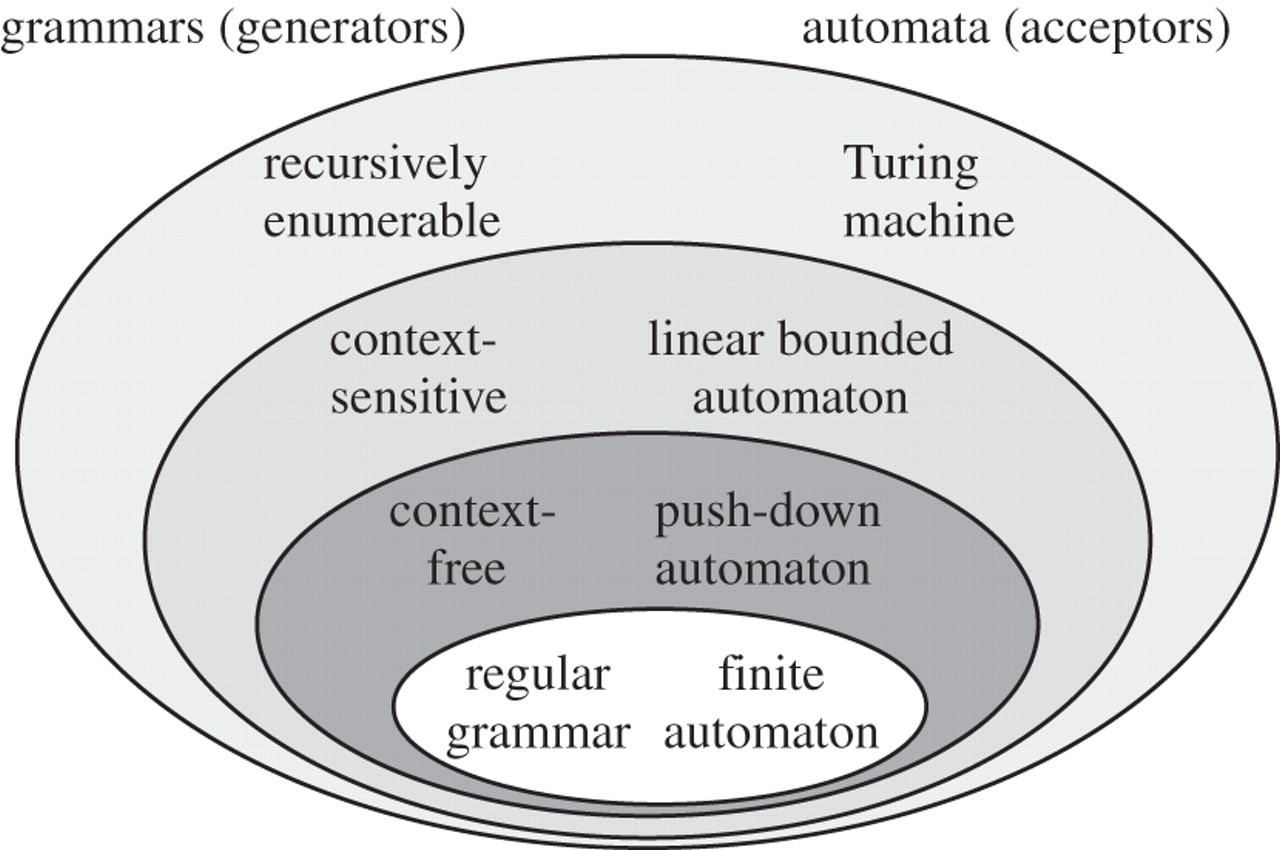
\includegraphics[width=0.75\textwidth]{./img/chom}
  \caption{Overzicht van de Chomsky-hi\"erarchie}
\end{figure}

\begin{quest}[$A_{TM}$ is niet beslisbaar]
	Bewijs dat $A_{TM}$ niet beslisbaar is en steun daarbij niet op de stelling van \textit{Rice}. Zou het helpen als het toegelaten was op de stelling van \textit{Rice} te steunen? Is $A_{TM}$ herkenbaar? Co-herkenbaar?
\end{quest}

We hebben het hier over het acceptatieprobleem voor Turingmachines. We noemen de taal $A_{TM}$ met de volgende formele definitie. Informeel is elk element een tuple met het eerste element een ge\"encodeerde Turingmachine die de string $s$, het tweede element, accepteert.
\begin{center}
	$A_{TM} = \{ <M,s> |$ \textit{$M$ is een Turingmachine en} $ s \in L_M\}$
\end{center}

\subsubsection*{$A_{TM}$ is niet beslisbaar}
\begin{proof}
	Stel er bestaat een beslisser $B$ voor $A_{TM}$. De werking van $B$ kan op de volgende manier formeel gedefinieerd worden.

	\begin{pushcenter}
		$B(<M,s>)$ \textit{is accept als $M$ $s$ accepteert en anders reject}
	\end{pushcenter}

	$B$ weigert dus indien $M$ de input $s$ weigert of wanneer $M$ in een oneindige lus zit.
	We construeren nu een contradictie machine $C$ met de eigenschap om telkens het tegenovergestelde te accepteren (of te weigeren) van $B$. $C$ neemt daarbij enkel Machine $M$ als input en accept indien $M$ de string representatie van zichzelf accepteert. We kunnen dit op de volgende manier formeel schrijven.

	\begin{pushcenter}
		$\forall$ \textit{Turingmachine $M:$ $C(<M>) = \neg (B(<M,M>))$}
	\end{pushcenter}

	Daarbij is $\neg accept = reject$ en $\neg reject = accept$.  Neem nu voor $M$ hierboven $C$ zelf en vul deze in in $C$ en $B$ zelf. De volgende bewering komt tot stand.

	\begin{pushcenter}
		$C(<C>) = \neg (B(<C,C>))$
	\end{pushcenter}

	We zien dat $C$ zichzelf test. Indien $C$ zichzelf accepteert, dan is $\neg B(C,C) = C(C) = accept$. Aangezien $C$ $C$ accepteert, moet $B(C,C) = accept$ en dus $\neg B(C,C) = reject$. Contradictie.
	\\\\
	Conclusie: $C$ kan niet bestaan. Indien $B$ bestaat kan $C$ wel bestaan, dus $B$ bestaat ook niet. $A_{TM}$ is dus niet beslisbaar.
\end{proof}

\subsubsection*{De stelling van Rice}

\begin{theorem}[Stelling van Rice]
	Voor elke niet-triviale, taal-invariante eigenschap $P$ van Turingmachines geldt dat $Pos_P$ (en ook $Neg_P$) niet beslisbaar is.
\end{theorem}

Met deze stelling zouden we het hele bewijs kunnen inkorten. Door een niet-triviale, taal-invariante eigenschap $P$ te vinden van alle Turingmachines die $s$ herkennen, hebben we meteen aangetoond dat de taal in kwestie, $A_{TM}$ niet beslisbaar is.\footnote{Voor meer informatie over het bewijs, zie het laatste hoofdstuk.} Deze taal komt dan overeen met $Pos_P$. Een eigenschap van $<M,s>$ is bijvoorbeeld dat $M$ $s$ accepteert. $Pos_p = A_{TM}$ en dus is $A_{TM}$ niet beslisbaar.

\subsubsection*{$A_{TM}$ is herkenbaar}
\begin{proof}
	De herkenner $A$ voor $A_{TM}$ laat, met input $<M,s>$, $M$ lopen op $s$. Indien deze $M$ $s$ accepteert, dan accepteert $A$ zijn input. Indien deze de input $reject$, of gewoon niet stopt, dan zal $A$ deze ook niet accepteren. $A_{TM}$ is dus herkenbaar (ook hier zien we dat $A_{TM}$ niet beslisbaar is omdat deze kan blijven lopen).
\end{proof}

\subsubsection*{$A_{TM}$ is niet co-herkenbaar}
\begin{proof}
	$A_{TM}$ kan echter niet co-herkenbaar zijn. We bewijzen dit met contradictie. Indien $A_{TM}$ co-herkenbaar is, is deze dus herkenbaar en co-herkenbaar (zie vorig bewijs). Wanneer een taal deze beide eigenschappen bezit, is deze beslisbaar. Dit is een contradictie met het eerste bewijs.
\end{proof}


\end{document}
